\pagebreak
\null
\newpage
\section{Appendix}

In this section we provide the necessary definitions and mathematical concepts necessary to properly introduce the weak formulation of a differential problem, the Galerkin method and finally the Finite Element Method.\\

\paragraph{Linear operators, functionals and bilinear forms} A \textit{linear operator} $L: X\to X$ from the Hilbert space $(X, \norm \cdot)$ to itself is a map such that $L(\alpha x + \beta y) = \alpha L x + \beta L y$. A linear operator on a Hilbert space is \textit{continuous} (or {bounded}) if $\exists M:\ |Lx|\leq Mx$. $(x, \lambda)$ are called respectively \textit{eigenvector} and \textit{eigenvalue} of the linear operator $L$ if the image of $x$ through $L$ is a rescaling of $x$ of factor $\lambda$ i.e. $Lx = \lambda x$. The operator $L$ is called \textit{self-adjoint} if $\langle Lx, y\rangle = \langle x,Ly\rangle\ \  \forall x,y \in X$. Self-adjoint operators have two important properties: their eigenvalues are real, and two eigenvectors $x, y$ associated to different eigenvalues $\lambda, \mu$ are orthogonal. Indeed 
\begin{align*}
	\langle Lx, y\rangle &= \langle x,Ly\rangle,\\
	\langle \lambda x, y\rangle &= \langle x,\mu y\rangle,\\
	\lambda \langle  x, y\rangle &= \mu \langle x, y\rangle,
\end{align*}
that implies $ \langle  x, y\rangle = 0$. If the eigenvectors of a self-adjoint operator $L$ span the whole space $X$, then $L$ is called \textit{diagonalisable}.  A linear operator from a Hilbert space $X$ to $\mathbb R$ is called a linear \textit{functional} on $X$. A functional is bounded if $\exists M\geq 0: \ |Lx|\leq M\norm x$. The normed vector space made by the set of all linear bounded functionals on $X$ endowed with the norm $\norm L = sup_{v\in X}|Lv|/\norm v$ is called the \textit{dual} space of $X$ and is indicated with $X^\star$. An important property of linear functionals is that for every functional $L\in X^\star$, there exists a unique vector $u\in X$ such that
$$Lv = \langle u, v\rangle\quad \forall v\in X$$ 

A \textit{bilinear form} on the vector space $X$ is a map $a(\cdot, \cdot): X\times X\to F$ that is linear with respect to both arguments. It is said to be \textit{strongly coercive} if \\
$\exists\alpha>0:\ |a(x, x)|\geq \alpha \norm {x}^2$, and \textit{bounded} if $\exists M>0:\ |a(x, y)|\leq M \norm x \norm y$.

\paragraph{The Lax-Milgram theorem}
Before introducing the Galerkin method the last thing to do is to state the Lax-Milgram theorem, theorem that is the foundation of the FEM formulation.
\vspace{0.5cm}
\begin{theorem}[Lax-Milgram]
	If \(a(\cdot, \cdot)\) is a bounded and strongly coercive bilinear form on the Hilbert space \(X\),  $L\in X^\star$ is a linear bounded functional on $X$, there exist a unique solution $f$ to the following problem:
	\begin{equation}\label{eq:variational abstract problem}
	\text{Find }f\in X\text{ such that } a(f, v)=Lv \text{ for all } v \in X
	\end{equation}
	For such \(f\) one has \(\|f\| \leq \frac{1}{\alpha}\norm L\) where \(\alpha>0\) is the coercive constant \\\(a(v, v) \geq \alpha\norm v^{2} \forall v \in X.\)
\end{theorem} 
\vspace{0.5cm}
The Finite Element Method takes a PDE problem in strong form (\ref{eq:strong form}), reformulates it in the equivalent \textit{weak form} (\ref{eq:variational abstract problem}) through suitable definitions of $X, a(\cdot, \cdot), L$ and finally solves it through polynomial interpolation.
\subsubsection{Weak formulation of a PDE and Galerkin Method}

Galerkin's method is a method to approximate the solution $f$ of an infinite dimensional problem of the form (\ref{eq:variational abstract problem}) with the solution $f_h$ of a finite dimensional problem. Our goal is now to explain how to write a differential problem like 
\begin{align}\label{eq:strong form}
\begin{split}
&\text{Given a regular domain }\Omega\subset\mathbb R^2\text{ and } u\in C(\Omega)\text{, find }f\in C^2(\Omega) \text{ such that}\\
&\begin{cases}
-\partial_{x_1x_1}f(\mathbf x) - \partial_{x_2x_2}f(\mathbf x) = u(\mathbf x) & \mathbf x \in \Omega\\
f(\mathbf x) =  0& \mathbf x \in \partial \Omega
\end{cases}
\end{split}
\end{align}
in the form \ref{eq:variational abstract problem}. Let's multiply the differential equation times a sufficiently regular function $v$ that vanishes on $\partial \Omega$ and integrate on $\Omega$. We obtain
\begin{align}
\begin{cases}
-\int_{\mathbb S^2}\Delta f(\mathbf x)v(\mathbf x)d\mathbf x =\int_{\mathbb S^2} u(\mathbf x)v(\mathbf x)d\mathbf x &\quad \mathbf x \in \Omega\\
f(\mathbf x) =  0&\quad \mathbf x \in \partial \Omega
\end{cases}	
\end{align}
 Since the contribution of both $f$ and $v$ on the border $\partial \Omega$ is zero, \\$\int_{\partial \Omega}\nabla f \cdot \mathbf nv d\sigma=0$ and integrating by parts we get

\begin{equation}\label{eq:int by parts}
	\int_\Omega \nabla f(\mathbf x)\cdot\nabla v(\mathbf x) d\mathbf x = \int_\Omega  u(\mathbf x)\cdot v(\mathbf x)d\mathbf x
\end{equation}

By defining $a(f, v):=	\int_\Omega \nabla f(\mathbf x)\cdot\nabla v(\mathbf x) d\mathbf x $ and $Lv := \int_\Omega  u(\mathbf x)\cdot v(\mathbf x)d\mathbf x$ problem \ref{eq:int by parts} can be written in the form of equation \ref{eq:variational abstract problem}. It remains to choose a Hilbert space $(X, \langle\cdot,\cdot\rangle_X)$ such that (i) $X$ is "big enough" to include those functions such that all the integrals and derivatives in the problem \ref{eq:int by parts} is well defined. This means that $X$ must include those functions $f$ such that $f, \nabla f$ are in $L^2(\Omega)$ and has to be \textit{complete} with respect to the norm induced by the scalar product $\langle\cdot,\cdot\rangle_X$. At the same time $X$ must be (ii) "small enough" to include only those functions that vanish on the boundary of $\Omega$. and (iii) the hypothesis of the Lax-Milgram theorem are satisfied, i.e. $a(\cdot, \cdot)$ is actually bounded and coercive and $L$ is bounded and linear. It turns out that such an Hilbert space exists: it is called $H^1_0(\Omega)$, it contains all the functions $v$ such that $v\in L^2(\Omega), \nabla v\in L^2(\Omega)$ and it is endowed with the scalar product 
$$
\langle u, v\rangle_{H^1_0(\Omega)} = \int_\Omega u(\mathbf x)v(\mathbf x)d\mathbf x + \int_\Omega\nabla u(\mathbf x)\cdot \nabla v(\mathbf x) d\mathbf x
$$
$H^1_0$ contains only those functions that vanish on $\delta \Omega$ i.e. \\$f\in H^1_0(\Omega)\cap C(\Omega) \implies \left.f(\mathbf x)\right|_{\partial\Omega}=0$. This means that thanks to Lax-Milgram theorem the problem

\begin{equation}\label{eq:final variational form}
\begin{split}
	&\text{Given }u\in L^2(\Omega)\text{ find }f\in H^1_0(\Omega)\text{ such that }\\
	&\int_\Omega \nabla f(\mathbf x)\cdot\nabla v(\mathbf x) d\mathbf x = \int_\Omega  u(\mathbf x)\cdot v(\mathbf x)d\mathbf x\quad \forall v\in H^1_0(\Omega)
\end{split}
\end{equation}

\textit{has one and only one solution in} $H^1_0(\Omega)$. However, to have this result (existence and uniqueness of the solution) we had to pay the price of looking for the solution $f$ in $H^1_0(\Omega)$, a much bigger space than  $C^2(\Omega)$ that we had in the original, strong form of the problem. This means that our solution $f\in H^1_0(\Omega)$ to the problem (\ref{eq:final variational form}) could not be a solution to problem (\ref{eq:strong form}), because it could be not regular enough and the second derivative $\Delta f$ could not exist! Fortunately there are regularity results - that we omit here - that assure that if the forcing term $u$ is regular enough, then also the solution $f$ will be regular and thus the two formulations - strong and weak - of the problem are actually equivalent, and thus solving \ref{eq:final variational form} eventually leads to solving \ref{eq:strong form}.

Now that we know that a solution exists, we need to compute it! Computing it analytically is often impossible; Galerkin's method in a mathematical tool provide us a way to compute an approximation of the solution $f$. Take the weak problem \ref{eq:variational abstract problem}, but restrict the ambient space to be a finite dimensional subspace of $X$, say $V_h = \text{span}\{\phi_0, ..., \phi_{n-1}\}$. We write thus the Galerkin problem
\vspace{0.5cm}

\begin{equation}\label{eq:Galerkin problem}
		\text{Find }f_h\in V_h\text{ such that } a(f_h, v_h)=\langle u_h, v_h\rangle \text{ for all } u_h \in V_h
\end{equation}
\vspace{0.5cm}

The key property of the Galerkin method is that the error $f-f_h$ is orthogonal to $V_h$; thus by choosing a sequence of finite dimensional spaces that fill the original space $X$, we can get as close as we want to the continuous solution $f$.
To solve equation \ref{eq:Galerkin problem} we write $f_h, u_h, v$ as linear combinations of the basis $\{\phi_0, ..., \phi_{n-1}\}$
\begin{equation}\label{eq:basis functions}
	\begin{cases}
	f_h = f_0\phi_0 +  f_1\phi_1 + ...  f_{n-1}\phi_{n-1}\\
	u_h = u_0\phi_0 +  u_1\phi_1 + ...  u_{n-1}\phi_{n-1}\\
	v_h = v_0\phi_0 +  v_1\phi_1 + ...  v_{n-1}\phi_{n-1}
	\end{cases}
\end{equation}
 thus obtaining by linearity of the bilinear form and of the scalar product a linear system of equations in the $n$ coordinates of $f_h$
\begin{equation}\label{eq:Galerkin problem in the basis functions}
\text{Find }\mathbf f\in\mathbb R^n\text{ such that } \sum_{j=0}^{n-1}a(\phi_i, \phi_j)f_j=\sum_{j=0}^{n-1}\langle \phi_i, \phi_j\rangle u_j \text{ for all } i=0, ... n-1
\end{equation}

Defining the \textit{stiffness matrix} $(A)_{ij} = a(\phi_i, \phi_j)$ and the \textit{mass matrix} \\$(B)_{ij} = \langle \phi_i, \phi_j\rangle$ we can rewrite problem \ref{eq:Galerkin problem in the basis functions} in the following algebraic form
\begin{equation}\label{eq:Galerkin algebraic}
\text{Find }\mathbf f\in\mathbb R^n\text{ such that } A\mathbf f = B \mathbf u
\end{equation}
where $\mathbf f, \mathbf u$ are the vectors of coordinates of $f_h, u_h$ with respect to the basis $(\phi_i)$. 
\vspace{0.5cm}
\begin{remark}
	 If the basis functions $\phi_i$ are orthonormal, then the mass matrix $B$ is the identity matrix. Furthermore, the scalar product in the space $V_h$ of two functions $u_h, v_h$ is equal to the dot product defined by the mass matrix $B$ in $\mathbb R^n$ of the coordinate vectors
	\begin{equation}\label{eq:dot product}
	\langle u_h, v_h\rangle = \mathbf u^\intercal B \mathbf v
	\end{equation}
	The Galerkin method \ref{eq:Galerkin problem} is well posed by a straight-forward application of the Lax-Milgram theorem, and thus also the system \ref{eq:Galerkin algebraic} admits one and only one solution.
\end{remark}

 \subsubsection{The Finite Element Method}
 
  The Finite Element Method is a technique that let us construct a particular subspace $V_h$ in (\ref{eq:Galerkin problem}) through polynomial interpolation. Let's refer again to the problem \ref{eq:strong form} defined on the domain $\Omega\subset\mathbb R^2$ in figure \ref{fig:omega and mesh}. 
 \paragraph{Approximation of the domain $\Omega$}
\begin{figure}[h]
	\centering
	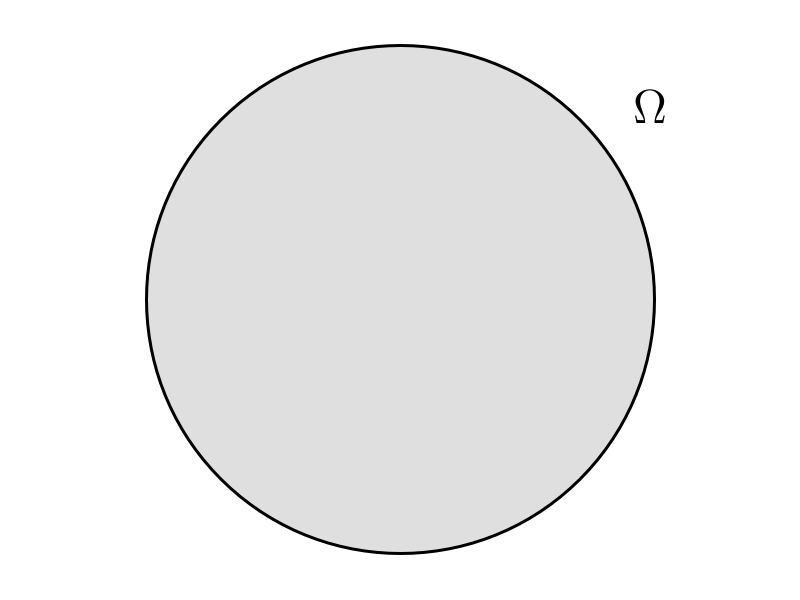
\includegraphics[width=0.4\textwidth]{figs/Chapter3/omega.png}
	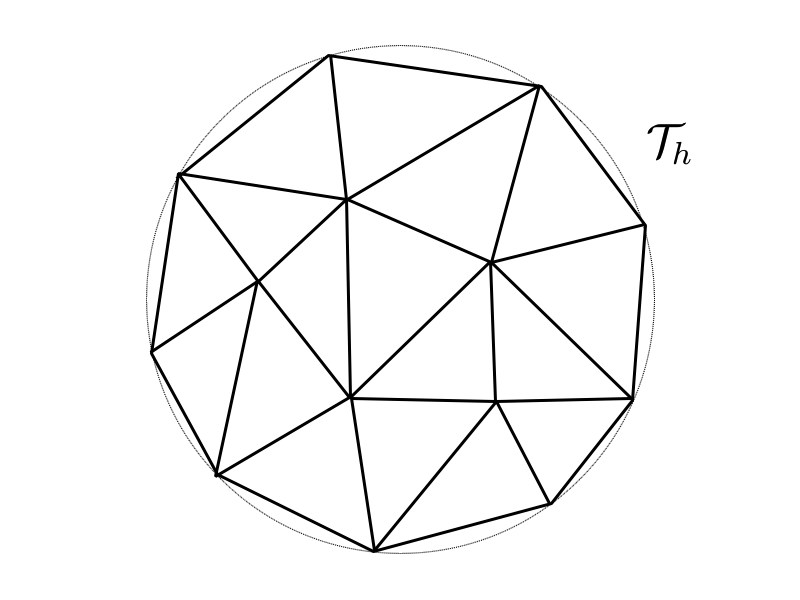
\includegraphics[width=0.4\textwidth]{figs/Chapter3/mesh.png}
	\caption{\label{fig:omega and mesh}The domain $\Omega$ and its approximation $\mathcal T_h$}
\end{figure}
First we need to construct a discretization of the continuous domain $\Omega$. In this example we take the triangulation in figure \ref{fig:omega and mesh} $\mathcal T_h = \left\{\tau_{k} : 1 \leq k \leq q\right\}$, where $h\in\mathbb R$ is a parameter such that every edge of the triangles $\tau_k\in\mathcal T_h$ is smaller than $h$. $\mathcal T_h$ is such that 
\begin{itemize}
	\item The elements \(\tau \in \mathcal{T}_h\) are closed subsets of \(\Omega\) with pairwise disjoint interior and \({\Omega}_h=\bigcup_{\tau \in \mathcal{T}_h} \tau\)
	\item The triangulation \(\mathcal{T}_h\) has no hanging vertices.
\end{itemize}

It's clear that by discretizing the continuous domain $\Omega$ we introduce a first source of errors in the method; however for simplicity we won't take this into account in the next discussion, and we will identify the domain $\Omega$ with the domain $\Omega_h$ covered by $\mathcal T_h$. The quality of the \textit{mesh} $\mathcal T_h$ is important for a good solution; a good quality mesh should avoid triangles with extreme angles and every triangle of $\mathcal T_h$ should look like as much as possible to an equilateral triangle. In figure \ref{fig:bad mesh} we see an example of a bad quality mesh: its triangles look very stretched; there are vertices that are shared by many triangles and vertices that are shared by very few. In figure \ref{fig:omega and mesh} we see a better mesh: there are no stretched triangles, and every vertex is shared by an almost constant number of triangles.
\begin{wrapfigure}{r}{0.3\textwidth}
	\begin{center}
		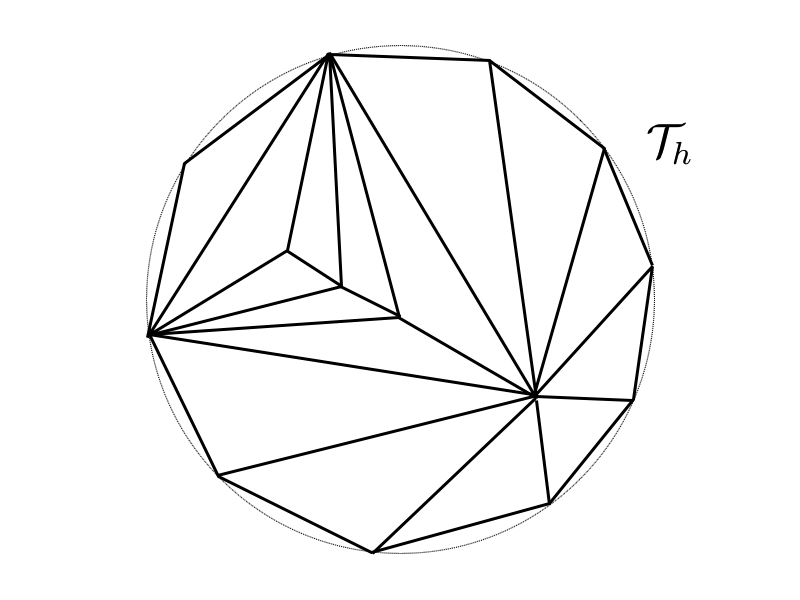
\includegraphics[width=0.4\textwidth]{figs/Chapter3/badmesh.png}
		\caption{\label{fig:bad mesh}A bad quality mesh}
	\end{center}
	
\end{wrapfigure}
\paragraph{Choosing $V_h$ and the basis functions $\phi_i$}

Beyond $X_h^1$, explained in section \ref{sec:Chapter3:FEM on the sphere}, other choices for $V_h$ are possible. A common choice is the space $X_h^{2}$ that is the space of all the piecewise second-order polynomials. In this case, since every second order polynomial in $\mathbb R^2$ has 6 degrees of freedom per each triangle $\tau_k$, meaning that we need to know its values in at least 6 different points on the triangle $\tau_k$ to uniquely identify it, the dimension of the space will grow (figure \ref{fig:elements}). A bigger space means that the approximation $f_h$ will be better, but we'll need more basis functions to define and thus it will result in a bigger linear system $Af = Bu$ and higher computational costs.
\begin{figure}[h!]
	\begin{center}
		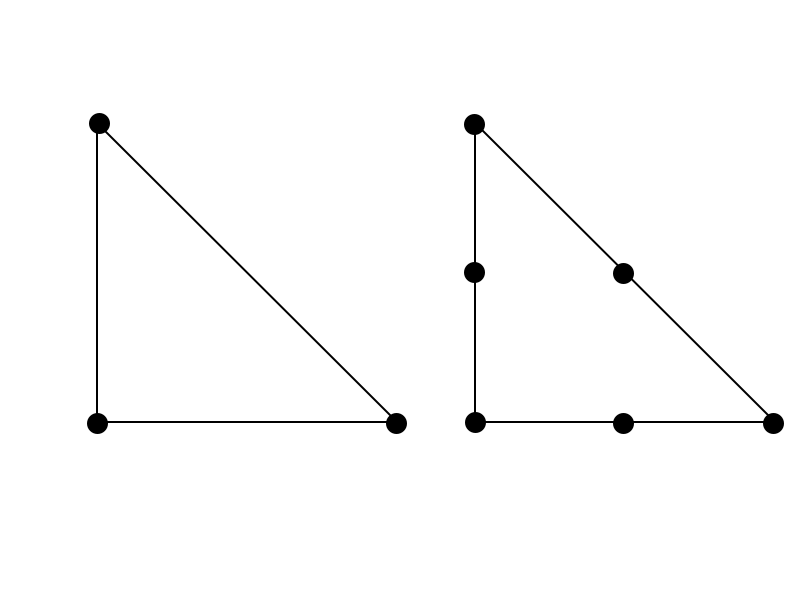
\includegraphics[width=0.4\textwidth]{figs/Chapter3/elemntsP1P2.png}
	\end{center}
	\caption{\label{fig:elements}The degrees of freedom (DOF) for $X_h^{1}$ and $X_h^{2}$ on a reference triangle}
\end{figure}
\paragraph{Assembling the stiffness and mass matrices}
Once defined the basis functions $\phi_i$, the FEM method constructs the stiffness matrix and the mass matrix $(A)_{ij} = a(\phi_i, \phi_j),\  (B)_{ij}=\langle\phi_i,\phi_j\rangle$ and solves the linear system \ref{eq:Galerkin algebraic} for the coefficients $f_i$ of the FEM solution $f_h$. An important fact to notice is both matrices $A$ and $B$ are \textit{sparse} and share the same sparsity pattern. Due to the form of the basis function $\phi_i$, the element $(i, j)$ of these matrices is different from zero only if the supports of the corresponding basis functions $(\phi_i, \phi_j)$ overlap, meaning that the vertices $(x_i, x_j)$ are connected by an edge of the mesh $\mathcal T_h$. In other words, the number of non-null entries of the $i-th$ row of $A$ and $B$ is equal to number of triangles of the mesh $\mathcal T_h$ that share the $i$th vertex i.e., the degree of the $i-th$ vertex.

\paragraph{About the boundary conditions}
	Note that the Dirichlet boundary conditions in the strong formulation of the differential problem \ref{eq:strong form} got transformed in the weak formulation \ref{eq:final variational form} as a condition on the ambient space $H_0^1(\Omega)$. Other kind of boundary conditions (Neumann, Robin for example) would not translate into the condition on the ambient space that functions must vanish on the border, but instead they would impose a different formulation of the bilinear form $a(\cdot, \cdot)$ or of the functional $L$. For this reason, Dirichlet boundary conditions are called \textit{essential} since translated into a condition on the ambient space and thus automatically satisfied from the FEM formulation; Neumann boundary conditions are called \textit{natural} since they transform into a different weak formulation through a modification of the bilinear form $a(\cdot, \cdot)$ and/or the functional $L$.

